\section{占有数表象}

\begin{quotation}
``科学中的想象力必须是明确的、确定的,不能只是一个模糊的假设。''\qquad 费曼
\end{quotation}

通过解微分方程,前面我们求解过线性谐振子问题。现在我们尝试发展一种代数方法求解,并介绍线性谐振子的占有数表象。

\subsection{线性谐振子的代数解法}

\index{Linear Oscillator: 线性谐振子}

线性谐振子的哈密顿量:

\begin{equation}
H = \frac{P^2}{2m} + \frac{m \omega^2 X^2}{2}
\end{equation}

这里的$X$和$P$分别是位置和动量算符,满足基础对易式:

\begin{equation}
\left[X, P \right] = i \hbar
\end{equation}

考虑到:

\begin{equation}
a^2 + b^2 = \left( a + ib \right) \left( a - ib \right) 
\end{equation}

我们可以尝试地把$\left( \frac{P^2}{2m} + \frac{m \omega^2 X^2}{2} \right)$也分成这样两部分,

\begin{eqnarray*}
{} & {} & \hbar \omega \left( \frac{P}{\sqrt{ 2m \hbar \omega }}  + i \sqrt{ \frac{m \omega }{2 \hbar} } X  \right) \left( \frac{P}{\sqrt{ 2m \hbar \omega }}  - i \sqrt{ \frac{m \omega }{2 \hbar} } X  \right)\\
{} & = & \left( \frac{P^2}{2m} + \frac{m \omega^2 X^2}{2} \right) + i \frac{\omega}{2} \left( XP - PX \right) \\
{} & = & \left( \frac{P^2}{2m} + \frac{m \omega^2 X^2}{2} \right) - \frac{\hbar \omega}{2}
\end{eqnarray*}

定义$a$和$a^\dagger$为:

\begin{eqnarray}\label{uv_eta_equals_1}
a &=& \frac{P}{\sqrt{ 2m \hbar \omega }} - i \sqrt{ \frac{m \omega }{2 \hbar} } X \\\label{uv_eta_equals11}
a^\dagger &=& \frac{P}{\sqrt{ 2m \hbar \omega }}  + i \sqrt{ \frac{m \omega }{2 \hbar} } X
\end{eqnarray}

我们可以证明这么定义的$a$和$a^\dagger$满足对易关系:

\begin{equation}
\left[ a, a^\dagger  \right] = 1
\end{equation}

使用$a, a^\dagger$,哈密顿量重新改写为:

\begin{equation}
H = \hbar \omega \left( a^\dagger a + \frac{1}{2} \right)
\end{equation}

那么$a^\dagger a$的含义是什么呢?首先它是个厄米算符,是可以对应物理量的,其次我们把$a^\dagger a$记做数算符$N$,假设它的本征值问题可以表示为:

\begin{equation}
N \left| n \right\rangle = n \left| n \right\rangle
\end{equation}

考虑对易式$\left[ N, a \right]$,利用$\left[ a, a^\dagger \right] = 1$,可得:

\begin{equation*}
\left[ N, a \right]  = \left[ a^\dagger a , a \right] = - a
\end{equation*}

我们把$\left[ N, a \right] $作用于$N$的本征态$\left| n \right\rangle$:

\begin{equation*}
\left( N a - a N \right) \left| n \right\rangle = N a \left| n \right\rangle - n a \left| n \right\rangle = - a \left| n \right\rangle
\end{equation*}

整理一下:

\begin{equation}
N a \left| n \right\rangle = (n -1) a \left| n \right\rangle
\end{equation}

这意味着对$a \left| n \right\rangle$而言,本征值$n$会减少1,在此意义下我们称$a$为湮灭算符\index{Annihilation operator: 湮灭算符}。但$a \left| n \right\rangle$不一定是归一的,假设$a \left| n \right\rangle = \gamma \left| n -1 \right\rangle$,我们有:

\begin{equation*}
\left\langle n \right| a^\dagger a \left| n \right\rangle = n = \gamma^2
\end{equation*}

因此:

\begin{equation}
a \left| n \right\rangle = \sqrt{n} \left| n -1 \right\rangle
\end{equation}

我们还可以考虑$N$和$a^\dagger$的对易式$\left[ N, a^\dagger \right]$,

\begin{equation*}
\left[ N, a^\dagger \right] = \left[ a^\dagger a , a^\dagger \right] = a^\dagger
\end{equation*}

我们把$\left[ N, a^\dagger \right] $作用于$N$的本征态$\left| n \right\rangle$:

\begin{equation*}
\left( N a^\dagger - a^\dagger N \right) \left| n \right\rangle =   N a^\dagger \left| n \right\rangle - n a^\dagger \left| n \right\rangle = a^\dagger \left| n \right\rangle 
\end{equation*}

整理一下,就是:

\begin{equation}
N a^\dagger \left| n \right\rangle = (n +1) a^\dagger \left| n \right\rangle
\end{equation}

这意味着对$a^\dagger \left| n \right\rangle$而言,本征值$n$会增加1,我们称$a^\dagger$为产生算符\index{Creation operator: 产生算符}。

假设$a^\dagger \left| n \right\rangle = \eta \left| n+1 \right\rangle$,$\left\langle n \right| a a^\dagger \left| n \right\rangle = n + 1 = \eta^2 $,因此:

\begin{equation}
a^\dagger \left| n \right\rangle = \sqrt{n + 1} \left| n+1 \right\rangle 
\end{equation}

~

现在的问题是$n$的取值范围是什么。考虑到:

\begin{equation}
\left\langle n \right| a^\dagger a \left| n \right\rangle = n
\end{equation}

是非负的,

\begin{equation}
n \ge 0
\end{equation}

那么$n$可以是分数吗,比如$n = \frac{1}{2}$?如果是这样的话,再湮灭一次,$n$就会小于0,这也是不合理的。

剩下的就只有$n = 0, 1, 2, ...$。$a^\dagger a$可以理解为占有数算符,本征值问题:$a^\dagger  a\left| n \right\rangle  = n\left| n \right\rangle $,$n$ 是占有数算符的本征值,$\left| n \right\rangle $是占有数算符的本征态,如以占有数算符的正交归一本征态$\left| n \right\rangle $为基矢,对应的表象就是占有数表象。

~

对$n = 0$而言,

\begin{equation}
a \left| 0 \right\rangle = 0
\end{equation}

线性谐振子的能量本征值是:

\begin{equation}
E_n = \left( n + \frac{1}{2} \right) \hbar \omega, n = 0, 1, 2, ...
\end{equation}

假设$\left| 0 \right\rangle$已经归一,能量本征矢是$\left| n \right\rangle$可表示为:

\begin{equation}
\left| n \right\rangle = \frac{ \left( a^\dagger \right)^n }{\sqrt{n !}} \left| 0 \right\rangle
\end{equation}

这里$\left| 0 \right\rangle$是基态,也叫真空态,对应0个$\hbar \omega$能量的激发。但真空态本身有个能量$\frac{\hbar \omega}{2}$,这是我们刚刚用不确定关系估算出来的,这个能量也叫零点能或真空涨落的能量\index{Zero-point energy: 零点能}。

$\left| 1 \right\rangle$对应只有1个能量激发$\hbar \omega$的态,$\left| 2 \right\rangle$对应有2个能量激发$\hbar \omega$的态……,$\left| n \right\rangle$对应有$n$个能量激发$\hbar \omega$的态……

\begin{figure}[htbp]
\begin{center}
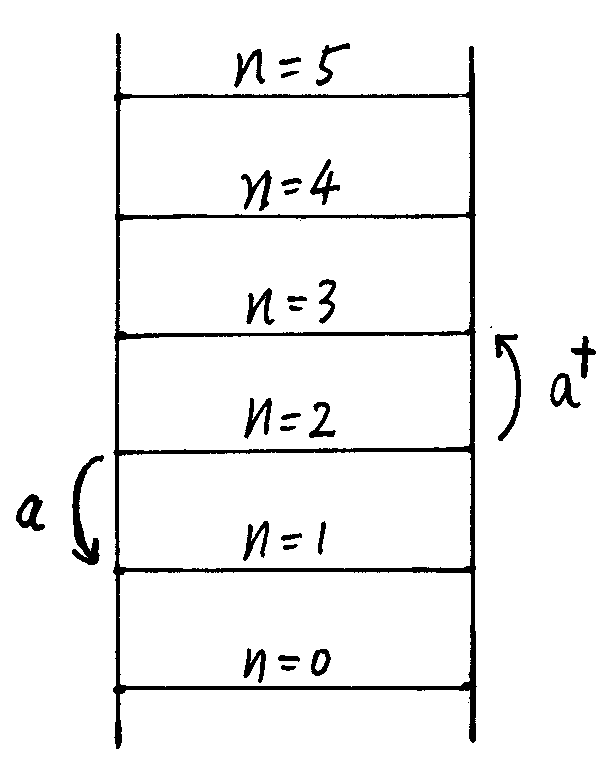
\includegraphics[width=5cm]{LinearOscillator/ladder.png}
\caption{能量的阶梯。}
\label{default}
\end{center}
\end{figure}

$E_n = \left( n + \frac{1}{2}  \right) \hbar \omega$构成了一个能量的台阶,每上一个台阶,就是多了个$\hbar \omega$能量的激发,相应地会多一份$\hbar \omega$的能量,当然第0级,或基态本身会有个非零的零点能$\frac{\hbar \omega}{2}$,因此这个能量的阶梯就是:

\begin{equation*}
\frac{\hbar \omega}{2}, \frac{3 \hbar \omega}{2}, \frac{5 \hbar \omega}{2}, \frac{7 \hbar \omega}{2}, ......
\end{equation*}

\subsection{uv变换}

恰当的线性变换可以使哈密顿对角化。下面介绍一种条理化的寻找变换系数的方法。

我们由线性谐振子的哈密顿出发:

\begin{equation*}
   H=\frac{p^2}{2m}+\frac{m\omega^2 x^2}{2}
\end{equation*}

计算运动方程:

\begin{eqnarray}
\frac{dx}{dt} &=& \frac{[x,H]}{i\hbar}=\frac{[x,p^2]}{2mi\hbar}=\frac{p}{m} \\
\frac{dp}{dt} &=& \frac{[p,H]}{i\hbar}=\frac{m \omega^2 [p,x^2]}{2i\hbar}=- m\omega^2x
\end{eqnarray}


这提示我们$x$随时间的演化与$p$有关,而$p$随时间的演化与$x$有关,为了“脱耦”我们把$x,p$组合起来,即定义:

\begin{eqnarray}
a &=& ux +vp \\
a^\dagger &=& u^* x + v^* p
\end{eqnarray}

使$a$(或$a^\dagger$)随时间的演化只与$a$(或$a^\dagger$)有关。这意味着线性变换$a = u x + v p$,使得哈密顿量$H(x, p )$取“对角化”的样子:

\begin{equation*}
H(x, p) = E a^\dagger a + Const.
\end{equation*}

这里$E$是$a$对应的激发能,Const.是一些与$a$, $a^\dagger$无关的常数。

$a$和$a^\dagger$还需满足对易关系:

\begin{equation}
[a, a^\dagger ]=1
\end{equation}

即假设激发是玻色子,得到:

\begin{equation}
[ux+vp,u^*x + v^*p] = (uv^*-u^*v)i\hbar=1
\end{equation}

这意味着:

\begin{equation}
u v^* - u^* v = - \frac{i }{\hbar}
\end{equation}

求解海森堡运动方程,$a$的运动将只与$a$有关:

\begin{equation}
\dot a = \frac{[a, H(a, a^\dagger)]}{i \hbar} = \frac{E}{i \hbar} a
\end{equation}

因此:

\begin{equation*}
\dot{a} =u \dot{x} + v \dot{p}=\frac{up}{m} - vm\omega^2x = \frac{E}{i \hbar}
(ux + vp)
\end{equation*}

解出:

\begin{equation*}
\frac{u^2}{v^2} = -m^2\omega^2
\end{equation*}

因此:

\begin{equation}
\frac{u}{v}=\pm im \omega
\end{equation}

把$u=\pm im\omega v$,代入:

\begin{equation*}
uv^* - u^*v = \frac{-i}{\hbar} = \pm i 2 m \omega |v|^2
\end{equation*}

取``+''无解,取``-''得到:$|v|^2=\frac{1}{2m\hbar\omega}$,即:

\begin{eqnarray}
u &=& -i \eta \sqrt{\frac{m \omega}{2\hbar}} \\
v &=& \frac{\eta}{\sqrt{2m\hbar \omega}}
\end{eqnarray}

其中$\eta$是任意相位因子,如果$\eta =1$,就得到前述$a$和$a^\dagger$的公式(\ref{uv_eta_equals_1}, \ref{uv_eta_equals11}):

\begin{eqnarray*}
a & = & -i \sqrt{ \frac{m \omega}{2 \hbar} } x + \frac{p}{ \sqrt{2m \hbar \omega} }\\
a^\dagger & = & i \sqrt{\frac{m \omega}{2 \hbar} } x + \frac{p}{\sqrt{2m \hbar \omega}}
\end{eqnarray*}

假设$\eta = e^{i \theta} $,$\theta \neq 0$。$\eta \neq 1$,$\theta \neq 0$相当于是做了个规范变换:

\begin{equation*}
\left( \begin{array}{c} a \\ a^\dagger \end{array} \right) \rightarrow \left( \begin{array}{c} \eta a \\  \eta^* a^\dagger \end{array} \right)
\end{equation*}

假设$\eta = i$,就得到常见的$a$和$a^\dagger$的表达式:

\begin{eqnarray}
a & = & \sqrt{\frac{m \omega}{2\hbar}} x + \frac{i}{\sqrt{2m\hbar \omega}} p \\
a^\dagger & = & \sqrt{\frac{m \omega}{2\hbar}} x - \frac{i}{\sqrt{2m\hbar \omega}} p
\end{eqnarray}

在此基础上,再将$x$, $p$表示为$a$, $a^{\dagger}$的形式\footnote{ 对一般的$\eta$:

\begin{eqnarray}
x & = & i \hbar (v^* a - v a^\dagger) \\
p & = & - i \hbar ( u^* a -u a^\dagger )
\end{eqnarray}}:

\begin{eqnarray}
x &=& \sqrt{\frac{\hbar}{ 2 m \omega} } (a + a^\dagger) \\
p &=& i \sqrt{ \frac{m \hbar \omega}{2} } (-a + a^\dagger)
\end{eqnarray}

把$x, p$代入哈密顿量中化简,得到:

\begin{equation}
H = \hbar \omega(a^{\dagger}a +\frac{1}{2})
\end{equation}

以上就是所谓uv变换,uv变换也叫波戈留波夫变换(Bogoliubov transformation)\index{Bogoliubov transformation: 波戈留波夫变换}。

~~

在海森堡绘景中,考虑$a(t) = e^{i Ht / \hbar} a(0) e^{- i Ht /\hbar}$随时间的演化:

\begin{equation}
\dot a = \frac{[a, H]}{i \hbar} = \frac{ \hbar \omega a }{i \hbar} = - i \omega a
\end{equation}

解此微分方程:

\begin{equation}
a(t) = a(0) e^{- i \omega t} 
\end{equation}

相应地,得到$a^\dagger$的表达:

\begin{equation}
a^\dagger(t) = a^\dagger(0) e^{i \omega t} 
\end{equation}

由此可得位置$x(t)$随时间的变化:

\begin{equation}
x(t) = \sqrt{\frac{\hbar}{ 2 m \omega}}  \left( a(0) e^{-i \omega t} + a^\dagger(0) e^{i \omega t}  \right) = \sqrt{\frac{\hbar}{ 2 m \omega}}  \left( a(0) e^{-i \omega t} + h.c.  \right) 
\end{equation}

上式中的$h.c.$是取前项$a(0) e^{-i \omega t}$的厄米共轭的意思。线性谐振子的占有数表象可用来描述声子(固体中晶格的集体振动),自旋波(固体中自旋取向的集体振动),光子(电磁辐射)等玻色子系统。

\subsection*{阅读与思考}


平行板电容器在辐射场真空态中存在吸引力的现象称为卡西米尔效应。考虑一个辐射的电磁场,
根据波粒二象性, 辐射场可以看作是光子气,
而光子气可看作是电磁辐射场的简谐振动。电磁场量子化后,
可把辐射场哈密顿写成二次量子化的形式(这里我们选取$\hbar=c=1$):


\begin{equation*}
    H=\sum\limits_k \omega_k (a_k^{+}a_k + 1/2)
\end{equation*}

\index{Casimir effect: 卡什米尔效应}

可见对每个振动模式$k$, 都有零点能(真空能)存在,
这个结果是引入场量子化后的自然结果。由于真空能量的存在可以带来实验可观测的物理效应——卡什米尔效应(casimir
effect)。


考虑一对距离为$a$的平行板电容器放在辐射场中, 边界条件为:
$E(0)=E(a)=0$ 。因此: $k_z = \frac{n \pi}{a}$,
可见随平行板距离的增大, 所允许的振动模式越多,
因此平行板电容器之间由于真空能量(Vaccum
energy)的存在而存在一种吸引力——卡什米尔力(Casimir
effect)。反之如果认为不存在真空能, 则没有这种力。

\index{Casimir force: 卡什米尔力}

\index{Vaccum energy: 真空能}

\begin{equation*}
 F=-\frac{\partial U(a)}{\partial a}
\end{equation*}


\index{Renormalization: 重整化}

在具体的计算过程中,
由于$U(a)$的积分(求和)是发散的。为得到收敛的结果,
数学上人为地引入一个切断因子,
这种作法在物理上叫做重整化(Renormalization)。最终计算可得:


\begin{equation*}
   \frac{F}{A}=-\frac{\pi^2}{240a^4}
\end{equation*}


更多请阅读: Zee A, \textbf{Quantum field theory in a nutshell}, pp65



\subsection*{练习}

\begin{itemize}

    \item 寻找合适的线性变换把哈密顿量:

\begin{center}
$H = E_0 a^\dagger a + E_1 (a^\dagger a^\dagger + a a)$
\end{center}

对角化,其中$E_0, E_1$是常数,$a, a^+$满足玻色子系统基本对易关系。

\item 声子的哈密顿量:

\begin{equation}
H = \sum\limits_q \frac{p_{-q}p_q }{2M} + \frac{M \omega_q^2 x_{-q} x_q}{2}
\end{equation}

并且$x, p$满足基础对易式:$[ x_q , p_{q'} ] = i \hbar \delta_{q,q'} $,请将上述哈密顿量对角化。

\end{itemize}




